\section{Metod}
Nedan beskrivs hur vi arbetar i gruppen samt hur vi kom fram till vald lösningsmetod. 

\subsection{Utvecklingsmetod}
Vi i grupp 2 strävar efter att träffas och arbeta tillsammans så mycket som möjligt. Detta för att kunna hjälpa varandra samt säkerhetsställa att alla har något att göra. Regelbundna möten hålls också för att stämma av vart vi befinner oss i projektet samt vad som ska göras. För att hålla ordning på alla aktiviteter under projektet använder vi en aktivitetstabell genom en webbtjänst där vi har delat upp aktiviteterna enligt följande: ska göras, pågående och färdiga. Varje aktivitet innehåller en kort beskrivning om vad som ska göras, hur mycket tid som kan läggas samt hur mycket tid som har lagts. 
\\
Vi arbetar inte efter någon speciell utvecklingsmetodik då vi kände att detta inte var nödvändigt för projektet.      

\subsection{Forskningsmetod}
När vi skulle välja lösningsalgoritm för konvexa kvadratiska problem fanns det två som var intressanta, Interior point method och Active set method. Metoderna återfinns i boken \emph{Numerical Optimization} och det var vår beställare Daniel som rekommenderade dessa. Enligt honom var båda ungefär lika komplicerade att implementera men trodde att ändå att Active set method kunde vara enklare. Detta gjorde att vi tillslut valde att gå vidare med den metoden. 
\\
För att förstå hur vi skulle gå tillväga med att implementera Active set method, löste vi först problemet tillsammans för hand. Detta gjorde att vi fick en klarare bild av hur algoritmen skulle se ut och hur den kunde delas upp i mindre funktioner.     

\subsubsection{Active set method}   
Metoden har fått sitt namn efter att den iterativt väljer vilka bivillkor i optimeringsproblemet som ska vara aktiva och söker efter den mängd aktiva bivillkor som ger ett globalt minimum. Nedanför visas pseudokod för algoritmen från \emph{Numerical Optimization}.

\begin{figure}[h]
\center
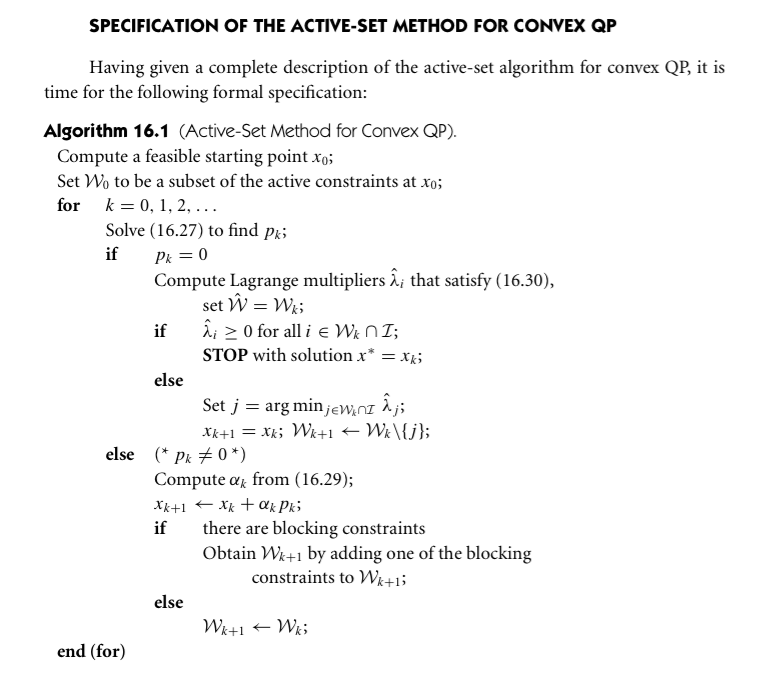
\includegraphics[scale=0.45]{grafik/algoritm.png}
\caption{Pseudokod för Active set method}
\endcenter
\end{figure}
